\chapter{Experimental results with spatio-angular microscope}
\label{sec:results}
\begin{summary}
Akzeptanzwinkel

Bleaching

Strukturierte Beleuchtung
Berechnung zu wenige beads

sample mit dichter 3d verteilung von beads
432r
3
2
33
3
23


3
2

2

2
2
2

2

2

2

2
2

\end{summary}

\section{Measuring acceptance angle for three different embedding
  media}
As one of the first attempts to use the spatio-angular illumination
system, I devised an experiment to determine the acceptance angle of a
microscope objective as a function of the embedding medium.

\begin{figure}[htbp]
  \centering
  \svginput{1}{tirf-exp}
  \caption{A fluorescent plane on a slide is embedded in oil, water or
    air. The thickness of the embedding medium is approximately
    $\unit[5]{\mu m}$. The focal plane SLM illuminates a disk with $\unit[30]{\mu
      m}$ diameter while a  window of $15\times 15$ pixels is scanned over the
    MMA. The window corresponds to a square with $\unit[210]{\mu m}$
    on the side as opposed to \unit[3.6]{mm} BFP diameter. 
% 200 px diameter on LCoS
% 15x15 px full diameter is D=2*(R=f*NA) f=164.5/63=2.61  NA=1.38
% D=3.6mm -> D/256*15 = 210 um
}
  \label{fig:tirf-exp}
\end{figure}



For the measurement a thin layer of fluorophores was applied with a
marker pen on three microscope slides. Furthermore, as a spacer, a
surrounding circle was painted with nail polish. After drying a drop
of immersion oil ($n=1.52$) or water ($n=1.33$) was added to two
samples. Then coverslips were added to all samples and sealed with
nail polish.

During \cma{scan pupil plane SLM} the measurement the focal plane SLM
projected a disk with $\unit[30]{\mu m}$ diameter on the fluorescent
plane. The illumination angle was varied by stepping a window of
$15\times 15$ pixels (equivalent to 1/17th of the pupil diameter) over
the pupil plane SLM.

For each angle, the sum of all the light on the camera is
recorded. The data is depicted in the three images in
\figref{fig:tirf-exp}.  These images contain a bright disk whose
diameter is growing with the index of the embedding medium. The center
of the disk corresponds to the optical axis of the
objective. Therefore pupil plane SLM is not exactly aligned with the
optical axis.  Points in the interior of the circle have an almost
constant intensity (residual fluctuations can be attributed to
non-uniformity of the illumination of the pupil plane SLM). For oil
immersion the diameter of the disk corresponds to the diameter of the
pupil.

If the index of the embedding medium is less than the index of the
immersion medium, then total internal reflection occurs on the
interface between coverslip and embedding medium for high incidence
angles. The excitation light can then no longer reach the
sample. Therefore, the disks in the plots for water and air are smaller.
{\color{red} FIXME winkel ausrechnen}


\section{Measuring light distribution by bleaching a fluorescent gel}
The above-described experiment allows only an indirect measure of the
effects of angular control in our microscope. Now I describe an
experiment where fluorophores in a slab of several microns thickness
are bleached. This allows a more direct measurement of the light
distribution in the sample by imaging the bleached region in a
confocal microscope.

As a sample we use a 4\% agarose gel containing fluorescently labeled
DNS plasmids. The exact sequence of the plasmids is irrelevant. They
only serve as carriers for the fluorophore (SYBR Save DNA gel stain,
Invitrogen). These samples are stable for several weeks and no
unbleached fluorophores return to bleached regions. The gel was chosen
and prepared by Florian R\"uckerl with whom I conducted this
experiment. We reported on this in \cite{Ruckerl}.

During the experiment the focal plane SLM displays three different
patterns (all dark, all bright, bright vertical bar) and the pupil
plane SLM displays eight different patterns (all dark, all bright, and
6 circular windows). The focal plane SLM was projected as far into the
middle of the gel layer as the working distance of the objective
allowed and an exposure series was mad overnight. Utilizing a
XY-stage, the sample was moved by \unit[0.4]{mm} between exposures.

% https://github.com/plops/cl-web-ui/commit/79ad04c61116b34aaf5f2422a3122a1d75ece890

The \cma{overall light efficiency} laser delivers a continuous beam of
\unit[473]{nm} wavelength with \unit[400]{mW} power. It is modulated
using an acousto-optic modulator (AOM) so that only during the camera
integration time (\unit[20]{ms}) and when the two SLM are in a defined
state light can excite the sample. The modulated beam has an average
power of \unit[15]{mW}. For this experiment I illuminate the rotating
micro-lens array and integrator rod directly (without fibre bundle). I
made this decision in the hope to reduce the necessary bleaching
time. In hindsight it would have been better to use the fibre
bundle. Behind the integrator tunnel there were still \unit[7]{mW}
average power and in front of the dichroic mirror of the microscope a
mere \unit[17]{uW} (with both SLM showing a white pattern).

\begin{figure}[htbp]
  \centering
  \svginput{1}{overview-bleach}
  \caption{The confocal measurements and images were kindly provided
    by Florian R\"uckerl (Institut Pasteur).}
  \label{fig:overview-bleach}
\end{figure}

\figref{fig:overview-bleach}~a) is a mosaic of confocal images in the
vicinity of the plane in the bleached gel where the focal plane SLM
was focused. The bleached areas form a pattern of $11\times 6$
exposures. The bleaching dose varies with the vertical direction as
indicated by the accumulated exposure times (consisting of numerous
\unit[20]{ms} exposures). 

FIXME translate
Erst bei 30s Bleachzeit ist ein deutliches in-focus bleaching erkennbar. 


Along the horizontal direction, different SLM patterns were
displayed. The two areas at both outer borders were bleached with full
angular and spatial exposure. The next column gives an indication of
how well both SLM can produce black as no bleaching pattern is evident
in these places.

The \cma{observed bleaching patterns1} central areas were all
displaying a vertical bar on the focal plane SLM while the pupil plane
SLM displayed a circular window, varying the incidence angle. The
first bar from the left was illuminated with all
angles. \figref{fig:overview-bleach}~b) shows a three-dimensional
representation of a confocal recording of the bleached
area. Unfortunately, three separate bundles are visible, indicating
insufficient uniformity of the illumination.

FIXME translate Die Unebenheiten sind auch nicht symmetrisch zur
optischen Achse, daher laufen die Buendel in leicht unterschiedlichen
Winkeln.

The images in \figref{fig:overview-bleach}~c) and d) show confocal
measurements of illumination with restricted angles. For this, a
circular window with radius $r=0.3$ was displayed on the pupil plane
SLM. Where the coordinates $\rho$ and $r$ are given relative to the
pupil radius --- for $\rho=1$ the window would be centered on the
periphery of the pupil, as indicated in the drawing
\figref{fig:overview-bleach}~e).

FIXME translate
Bei den rot markierten Zahlen im Bild handelt es sich um Markierungen,
die Nachtraeglich mit dem Confocal zu Orientierung eingebleicht
wurden.


\comment{
\jpginput{}{m_wf}{}
}

\section{Beads under spatio-angular illumination}

Das naechste Experiment ist der Bildgebung in einer biologischen Probe
nachempfunden. Hierfuer wurden 3um grosse Beads in einem Agarose-Gel
verteilt. Das Ziel ist, die Beads in einer ersten Aufnahme zu
lokalisieren und mit der Information ueber ihre dreidimensionale
Verteilung Pattern fuer focal plane SLM und pupil plane SLM zu
bestimmen um die Beads einzeln anzuleuchten und die Anregung von
out-of-focus beads zu vermeiden.

Zunaechst \cma{wide field baseline} zeige ich zum Vergleich in
\figref{fig:m_wf} eine Fokusserie mit 1 micron Schritten von wide
field Aufnahme bei der das maximale Feld in der Probe unter vollen
Winkeln beleuchtet wird. In diesen Aufnahmen sieht man wie mehrere
Beads nacheinander in-focus kommen. Leider liefert das Gel eine
relativ hohe Hintergrundfluoreszenz in der die verschwommenen Abbilder
von der Out-of-focus beads schnell nicht mehr unterscheidbar sind. Aus
diesem sparsen Datensatz kann man relativ einfach die 3D Verteilung
der Beads bestimmen. In einem Sample mit einer dichteren Verteilung
von Beads oder den Zellkernen in einem Embryo ist das jedoch nicht
mehr moeglich.


\begin{figure}[hbtp]
  \centering
  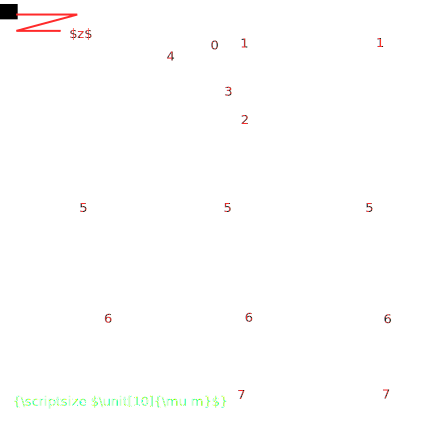
\includegraphics[width=12cm]{m_wf}
  \caption{Wide field stack of a three-dimensional distribution of
    yellow-green beads in agarose gel. Sampling in $z$ is
    $\unit[1]{\mu m}$.}
  \label{fig:m_wf}
\end{figure}

Dann \cma{optical sectioning} hilft eine Trennung von out-of-focus und in-focus
Fluoreszenslicht, wie sie mit strukturierter Beleuchtung moeglich
wird. \figref{fig:m_sec} zeigt das Ergebnis der Berechnung von
optischen Schnitten aus jeweils vier strukturiert beleuchteten
Rohbildern in \figref{fig:m_phase} in the Appendix on page
\pageref{fig:m_phase}.  Die Schnitte zeigen relativ praegnante
vertikale Rekonstruktionsartefakte, die bei Verwendung der HiLo
Rekonstruktion vermieden werden koennen. In lebenden Samplen wuerde
diese Methode ausserdem zu bevorzugen sein, weil sie nur zwei
Rohaufnahmen braucht.

Fuer \cma{bead localization} die Lokalisierung der Beads stoeren die
Artefakte jedoch nicht. Ich ermittelte die Mittelpunkte der Beads
durch bestimmung der lokalen maxima nach anwendung eines auf die beads
angepassten drei-dimensionalen difference of gaussian filters und das
ergebnis ist im inlay in \figref{fig:m_sec} geplottet. Die Beads
wurden automatisch vom Algorithmus numeriert.

\begin{figure}[hbtp]
  \centering
  \svginput{1}{m_sec}
  \caption{Computationally sectioned images. Note that two beads (4
    and 7) are very close to the border of the field of view and not
    fully illuminated.}
  \label{fig:m_sec}
\end{figure}

Ausgehend vom 3D modell masken fuer focal plane SLM zur individuelle
beleuchtung der beads erstellt und zu jeder dieser masken wird
automatisch eine maske fuer den pupil plane SLM erzeugt. 



\begin{figure}[hbtp]
  \centering
  \svginput{1}{angular-beads}
  \caption{Spatio-angular controlled illumination of the beads from
    \figref{fig:m_sec}. The top left image shows bead number zero and
    so forth, the second image in the top shows bead number one and so
    on. The LCoS selectively illuminates the target bead and the MMA
    displays the pattern shown in \figref{fig:m_bfp_co}.}
  \label{fig:m_ang}
\end{figure}


\begin{figure}[!hbt]
  \centering
  \svginput{1}{montage-ang}
  \caption{}
  \label{fig:montage-ang}
\end{figure}




%%% Local Variables: 
%%% mode: latex
%%% TeX-master: "kielhorn_memi"
%%% End: 
